\begin{frame}{Tìm kiếm lân cận}
  \begin{itemize}
    \item Lân cận
    \item Tối ưu địa phương
    \item Tiêu chí chấp nhận nghiệm
    \item Điều kiện dừng
  \end{itemize}
\end{frame}

\begin{frame}{Tìm kiếm lân cận rộng}
  \begin{figure}[H] % places figure environment here   
    \centering % Centers Graphic
    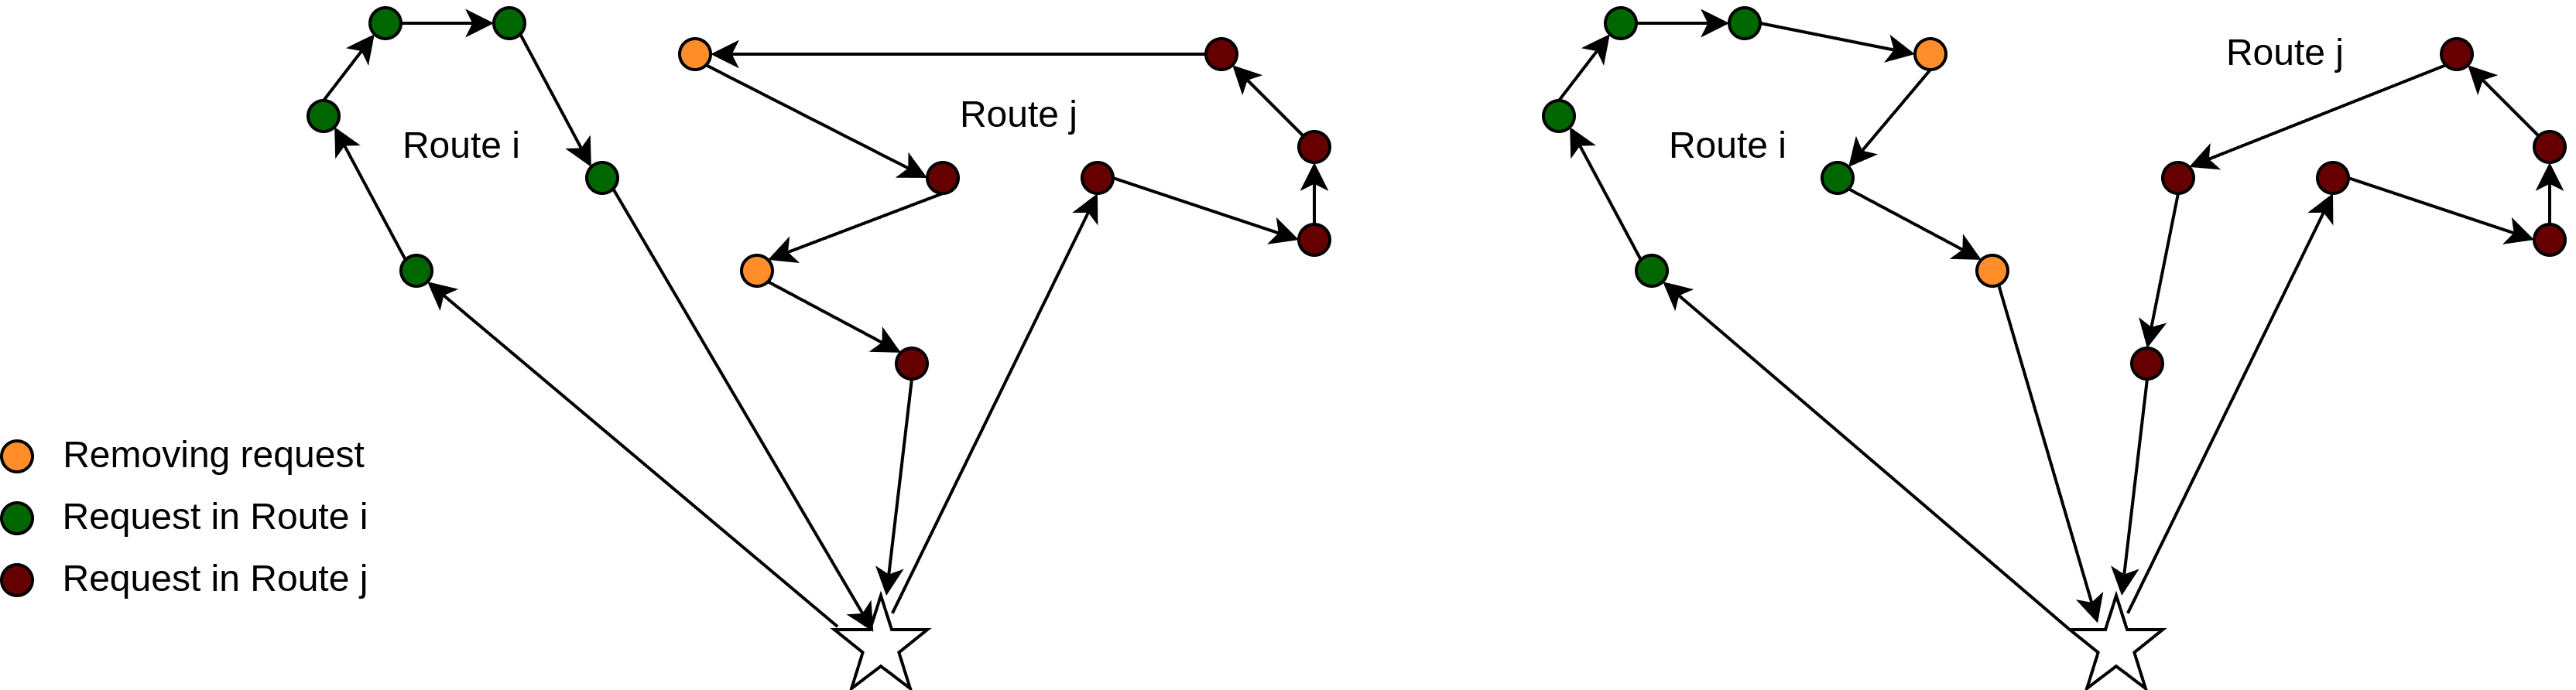
\includegraphics[width=0.9\textwidth]{figures/ALNS-paradim.png} 
    % \includesvg[scale=1]{figures/core-object}
    \caption{Lược đồ LNS} 
    \label{fig:lns_paradim}
  \end{figure}  
\end{frame}

\begin{frame}{Tìm kiếm lân cận rộng (\textit{LNS})}
  \begin{figure}[H] % places figure environment here   
    \centering % Centers Graphic
    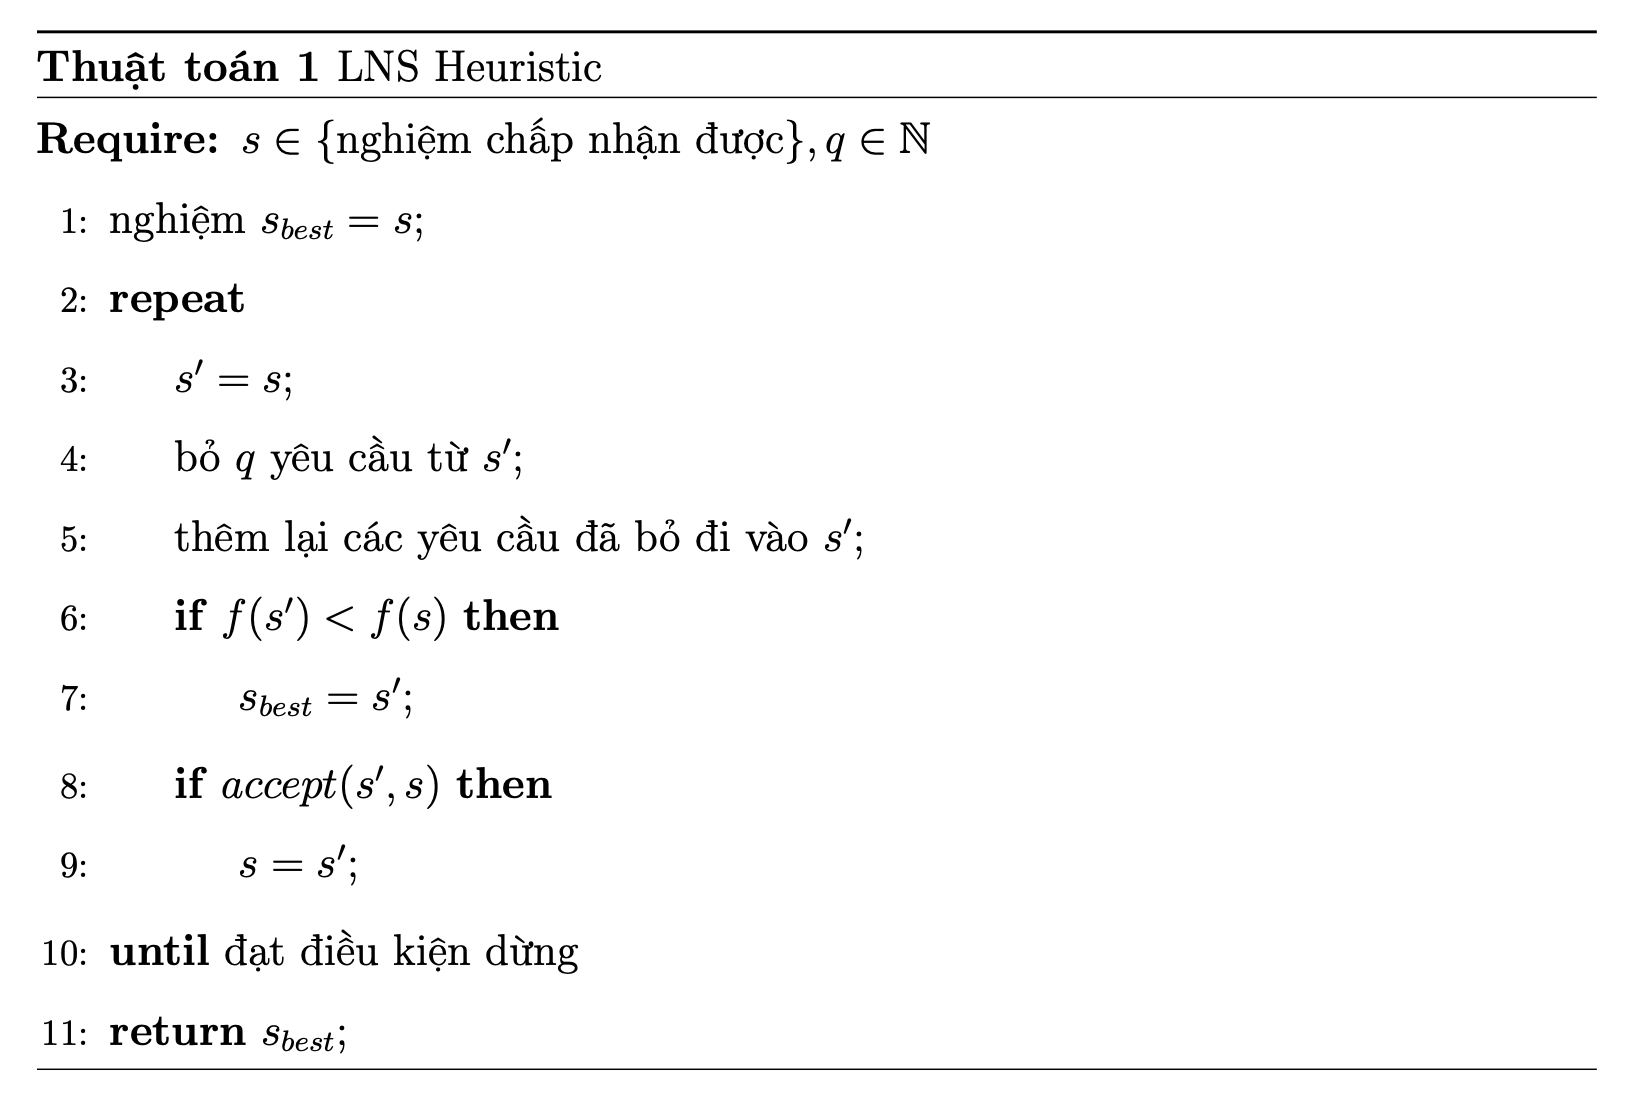
\includegraphics[width=0.8\textwidth]{figures/pr_LNS.png} 
    % \includesvg[scale=1]{figures/core-object}
    \caption{Mã giả LNS} 
    \label{fig:lns_pseudo}
  \end{figure} 
\end{frame}

\begin{frame}{LNS - Thuật toán hủy}
  % \begin{itemize}
  %   \item Xóa yêu cầu tệ nhất
  %   \item Xóa ngẫu nhiên
  %   \item Thuật toán xóa Shaw
  %   \item Thuật toán xóa tuyến tệ
  % \end{itemize}
  \begin{block}{Xóa yêu cầu tệ nhất}
  \end{block}
  \begin{block}{Xóa ngẫu nhiên}
  \end{block}
  \begin{block}{Thuật toán xóa Shaw}
  \end{block}
  \begin{block}{ Thuật toán xóa tuyến tệ}
  \end{block}
\end{frame}

\begin{frame}{LNS - Thuật toán hủy}
  \begin{block}{Xóa yêu cầu tệ nhất}
    \begin{itemize}
      \item Mảng $L$: sắp xếp các yêu cầu theo thứ tự giảm dần của chi phí (sau khi bỏ đi yêu cầu đó).
      \item Chọn một số ngẫu nhiên $y \in (0,1)$.
      \item Xóa yêu cầu $r = L[y^p|L|]$.
    \end{itemize}
  \end{block}
\end{frame}

\begin{frame}{LNS - Thuật toán hủy}
  \begin{block}{Xóa tuyến tệ nhất}
    Chi phí trung bình trên mỗi yêu cầu với nhiễu
    \begin{equation}
      \label{eq:destroy_route}
      \text{avg\_cost}(r, s) = \frac{\text{cost}(r, s)}{\text{size}(r)-1} + \lambda \phi d_{max}
    \end{equation}
    với $r$ là tuyến được chọn, $\text{cost}(r,s)$ là chi phí của tuyến $r$ trong nghiệm $s$, $\text{size}(r)$ là số phần tử của tuyến $r$, $\lambda$ là hệ số nhiễu, $\phi$ là một số ngẫu nhiên trong khoảng $(0,1)$, $d_{max}$ là khoảng cách lớn nhất trong tập yêu cầu.
    
    Xóa đi tuyến có chi phí trung bình trên mỗi yêu cầu lớn nhất và có số yêu cầu nhỏ hơn số yêu cầu trung bình trên mỗi tuyến (với một ngưỡng nhất định).
  \end{block}
\end{frame}

\begin{frame}{LNS - Thuật toán hủy}
  \begin{block}{Phương pháp xóa Shaw}
    Chỉ số độ tương đồng 
    \begin{equation}
      \label{eq:shaw_related}
      R(i,j) = \varphi d_{ij} + \chi |t_{i}-t_{j}| + \psi|l_i - l_j|
    \end{equation}
    với $d_{ij}$ là khoảng cách từ $i$ tới $j$, $t_i$ là thời gian khi đến địa điểm $i$, $l_i$ là tải của xe tại $i$.
  \end{block}
\end{frame}

\begin{frame}{LNS - Thuật toán hủy}
  \begin{figure}[H] % places figure environment here   
    \centering % Centers Graphic
    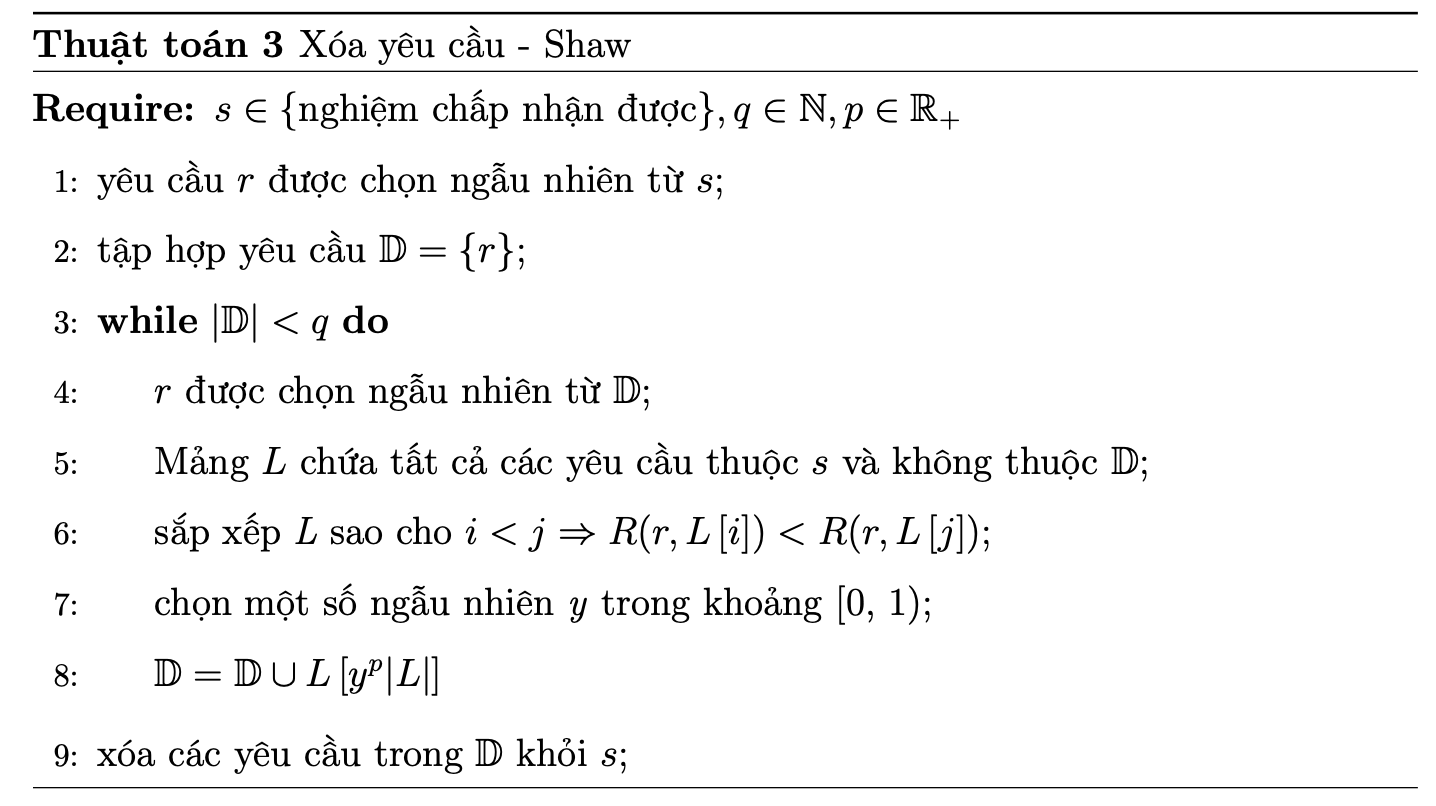
\includegraphics[width=1\textwidth]{figures/des_shaw.png} 
    % \includesvg[scale=1]{figures/core-object}
    \caption{Thuật toán xóa Shaw} 
    \label{fig:shaw_pseudo}
  \end{figure} 
\end{frame}

\begin{frame}{LNS - Thuật toán sửa}
  % \begin{itemize}
  %   \item Chèn yêu cầu tham lam (với nhiễu)
  %   \item Heuristic hối tiếc
  % \end{itemize}  
  \begin{block}{Chèn yêu cầu tham lam (với nhiễu)}
  \end{block}
  \begin{block}{Heuristic hối tiếc}
  \end{block}
\end{frame}

\begin{frame}{LNS - Thuật toán sửa}
  \begin{block}{Chèn yêu cầu tham lam}
    \begin{itemize}
      \item Khi chèn thêm yêu cầu $u$ và giữa hai yêu cầu $i$ và $j$ trong tuyến $k$ thì chi phí tăng thêm là $\Delta f_{u, i, j, k} = d_{iu} + d_{uj} - d_{ij}$.
      \item Chèn thêm yêu cầu vào vị trí làm tăng ít chi phí nhất.
      \item Có thể thêm nhiễu vào hàm tăng chi phí.
      \begin{equation}
        \Delta f_{u, i, j, k} := \Delta f_{u, i, j, k} + \lambda p d_{\text{max}}
      \end{equation}
      với $d_{\text{max}}$ là khoảng cách lớn nhất giữa hai yêu cầu, $p$ là một số ngẫu nhiên trong khoảng $(-1,1)$ và $\lambda$ là một hằng số điều khiển.
    \end{itemize}
  \end{block}
\end{frame}

\begin{frame}{LNS - Thuật toán sửa}
  \begin{block}{Heuristic hối tiếc}
    \begin{itemize}
      \item Đặt $x_{ik} \in \{1, ..., m\}$ là biến biểu diễn tuyến đường cho yêu cầu $i$ có chi phí chèn thêm vào thấp thứ $k$.
      \item Giá trị \textit{regret} $c_i^* = \Delta f_{i, x_{i2}} - \Delta f_{i, x_{i1}}$.
      \item Chọn ra yêu cầu $i$ thỏa mãn $\max_{i \in V \setminus \{0\}} \{c_i^*\}$ và chèn vào vị trí tương ứng.
      \item Mở rộng regret-k, chọn yêu cầu thỏa mãn
      \begin{equation}
        \max\limits_{i \in V \setminus \{0\} } \{ \sum_{j=1}^k (\Delta f_{i, x_{ij}} - \Delta f_{i, x_{i1}}) \}.
    \end{equation}
    \end{itemize}
  \end{block}
\end{frame}

\begin{frame}{LNS - Tiêu chí chấp nhận nghiệm}
    \begin{block}{Bước ngẫu nhiên - Ramdom Walk}
      Mọi nghiệm $s'$ đều được chấp nhận.
    \end{block}
    \begin{block}{Chấp nhận tham lam - Greedy Acceptance}
      Nghiệm $s'$ được chấp nhận nếu chi phí của nó là nhỏ hơn so với nghiệm hiện tại.
    \end{block}
    \begin{block}{Mô phỏng luyện kim - Simulated Annealing}
      Mọi nghiệm cải thiện $s'$ được chấp nhận. Nếu $c(s') > c(s)$ thì $s'$ được chấp nhận với xác suất $\exp \{ \frac{c(s) - c(s')}{T} \}$ với $T$ là nhiệt độ. Nhiệt độ $T$ giảm sau mỗi vòng lặp với một hệ số $\Phi$.
    \end{block}
\end{frame}

\begin{frame}{LNS - Tiêu chí chấp nhận nghiệm}
  \begin{block}{Chấp nhận với ngưỡng - Threshold Acceptance}
    Nghiệm $s'$ được chấp nhận nếu $c(s') - c(s) < T$ với $T$ là ngưỡng, ngưỡng này được giảm sau mỗi vòng lặp với hệ số $\Phi$.
  \end{block}
  
  \begin{block}{Đại hồng thủy - Great Deluge Algorithm}
    Nghiệm $s'$ được chấp nhận nếu $c(s') < L$ với một ngưỡng $L$, ngưỡng này chỉ giảm nếu nghiệm được chấp nhận, và giảm với hệ số $\Phi$.
  \end{block}
\end{frame}

\begin{frame}{Tìm kiếm lân cận rộng thích ứng (\textit{ALNS})}
  \begin{figure}[H] % places figure environment here   
    \centering % Centers Graphic
    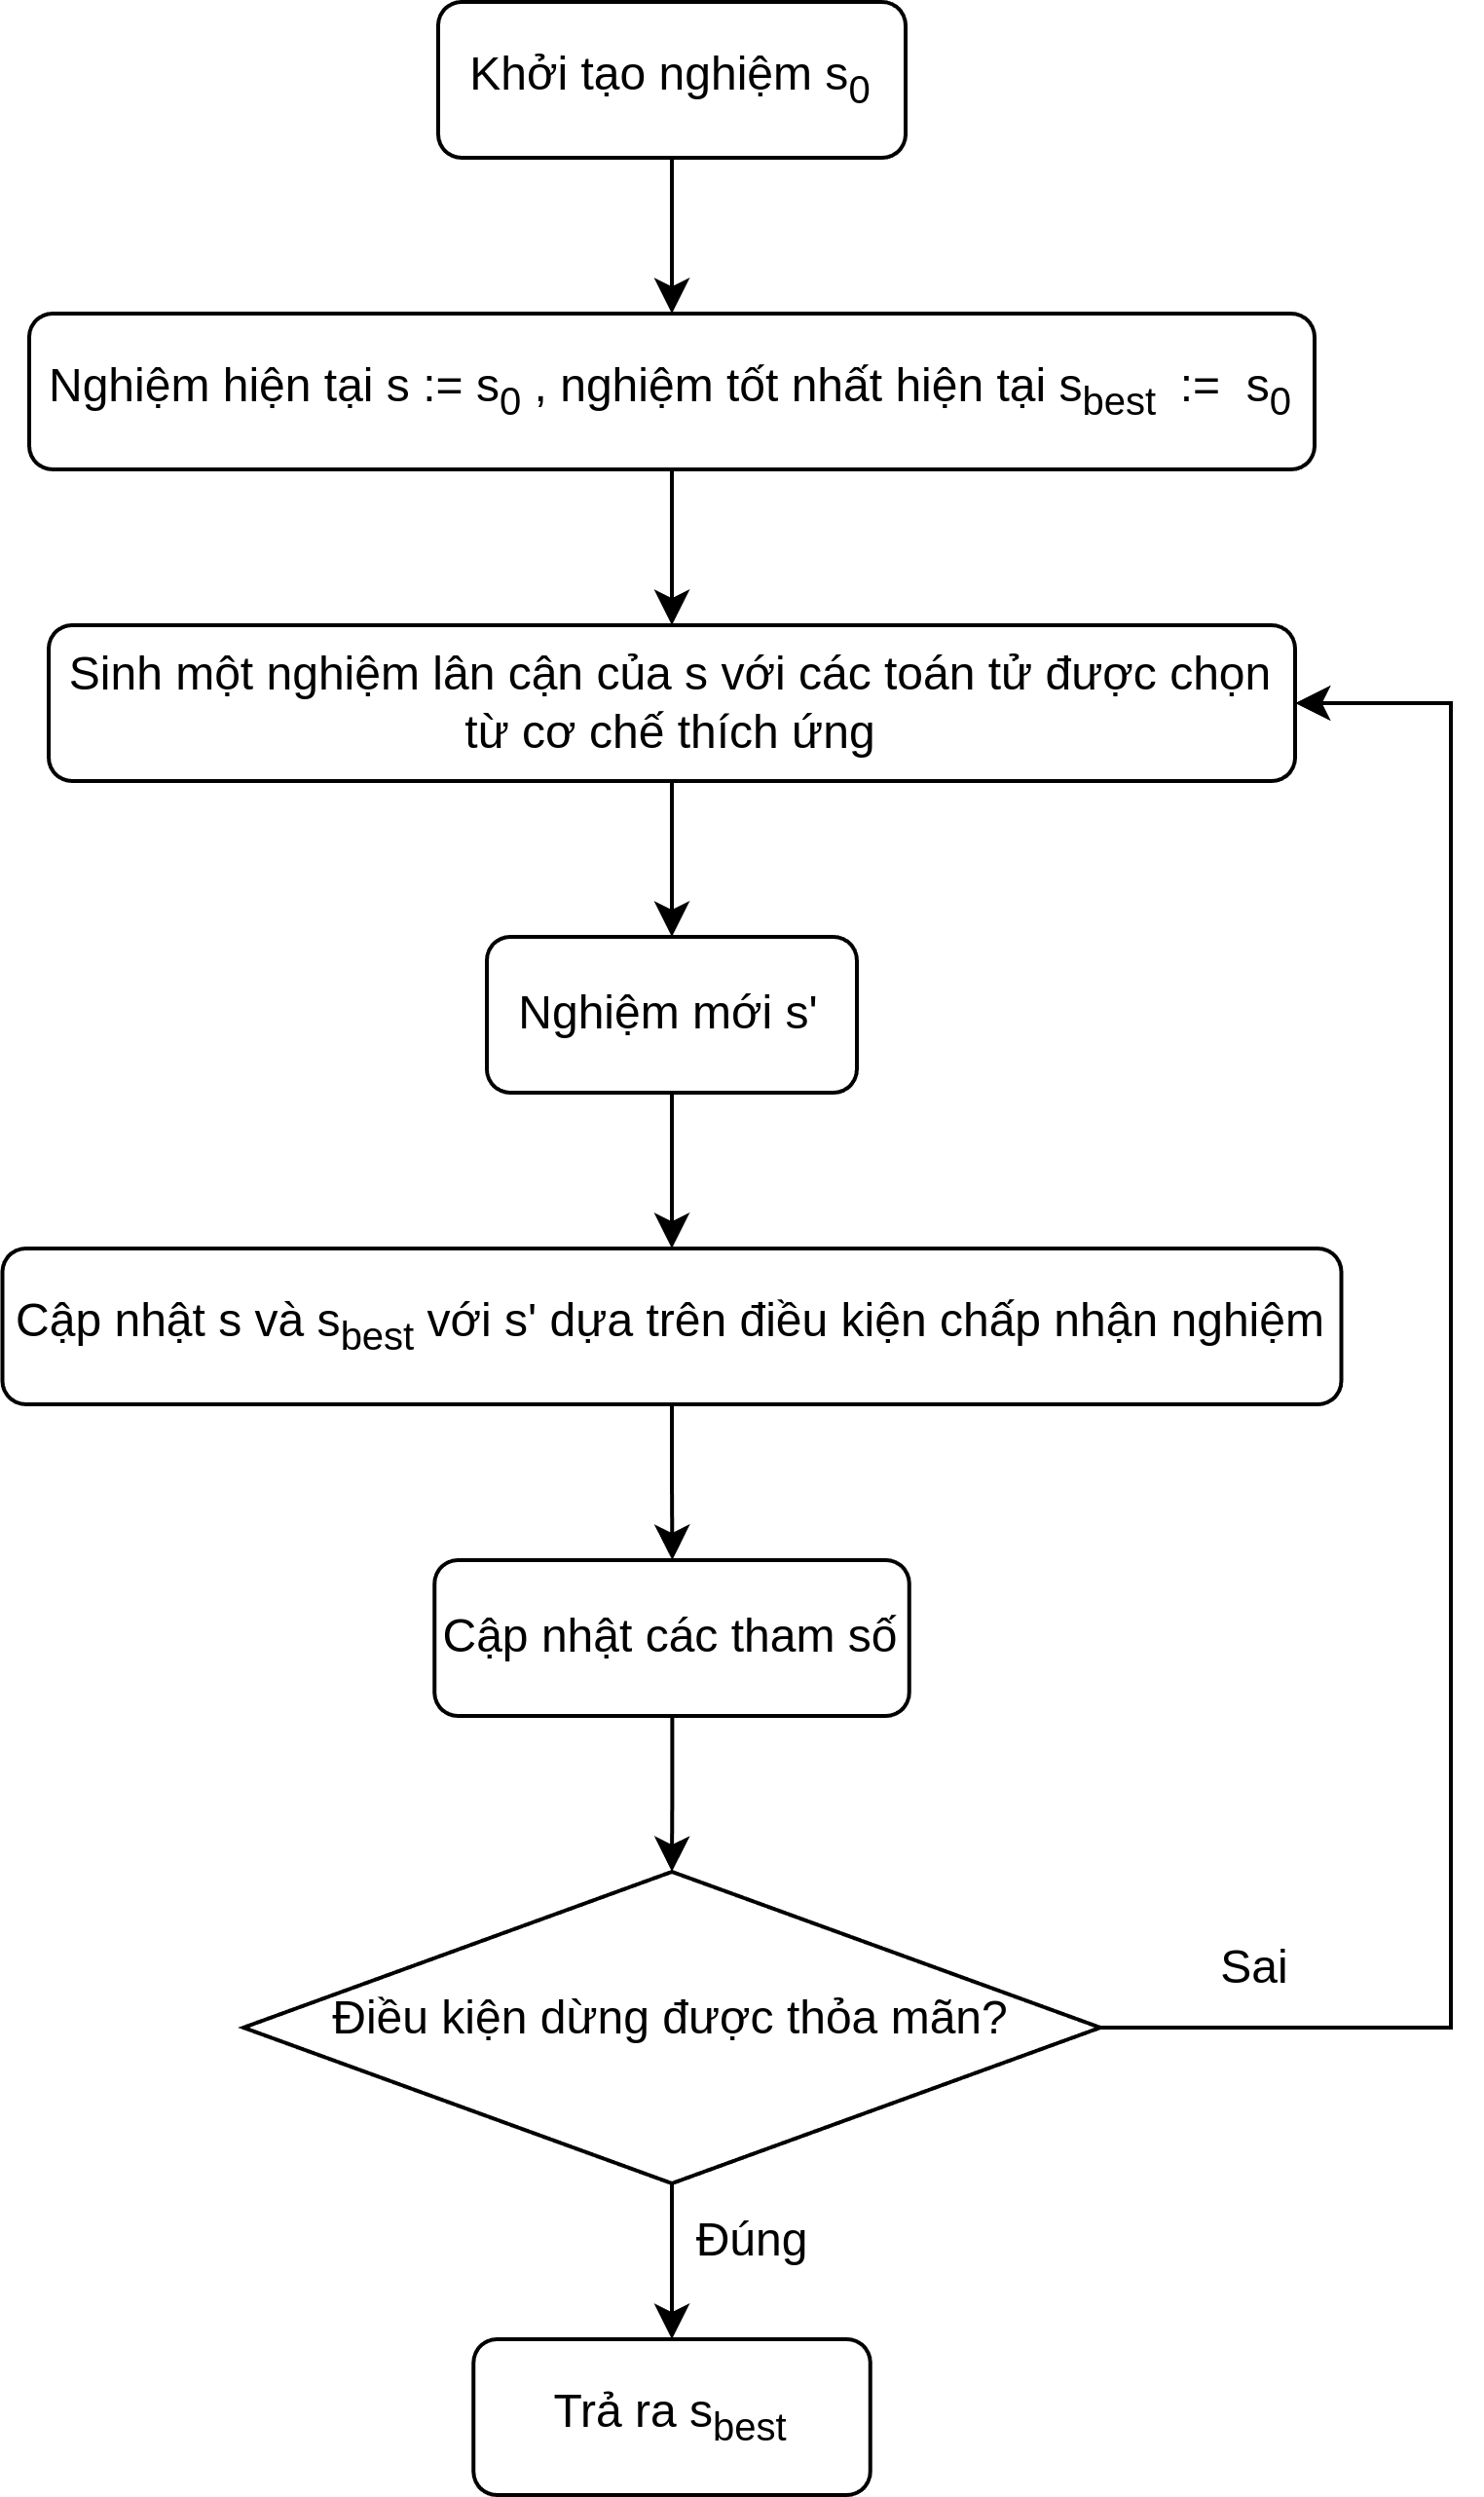
\includegraphics[width=0.3\textwidth]{figures/ALNS-flowchart.png} 
    % \includesvg[scale=1]{figures/core-object}
    \caption{Lược đồ chính của ALNS} 
    % \label{fig:fg_02}
  \end{figure}
\end{frame}

\begin{frame}{ALNS - Lựa chọn thuật toán}
  \begin{block}{Lựa chọn thuật toán hủy và thêm lại}
    Gán cho mỗi heuristic một trọng số khác nhau và sử dụng nguyên tắc "bánh xe lựa chọn". Nếu có $k$ heuristic với trọng số $w_i, i \in \{1,...,k\}$, ta chọn heuristic $j$ với xác suất
    \begin{equation}
      \label{eq:select}
      p_j = \frac{w_j}{\sum_{i=1}^k w_i}.
    \end{equation}
  \end{block}
\end{frame}

\begin{frame}{ALNS - Điều chỉnh tham số tự động}
  \begin{itemize}
    \item Trọng số được điều chỉnh mỗi khi có nghiệm mới được chấp nhận.
    \item Mỗi heuristic được gán điểm khác nhau và được điều chỉnh tùy thuộc vào tình huống.
    \item Cập nhật trọng số sau mỗi bước.
  \end{itemize}
\end{frame}

\begin{frame}{ALNS - Điều chỉnh tham số tự động}
  Điểm của mỗi heuristic được đặt là $0$ khi bắt đầu và được tăng thêm $\sigma_1, \sigma_2, \sigma_3$ tùy thuộc vào tình huống.
  \begin{itemize}
    \justifying
    \item $\sigma_1$ khi hành động xóa-chèn cuối cùng dẫn đến một nghiệm mới tốt hơn nghiệm tốt nhất toàn cục.
    \item $\sigma_2$ khi hành động xóa-chèn cuối cùng dẫn đến một nghiệm chưa được chấp nhận trước đó, chi phí tốt hơn chi phí của nghiệm hiện tại.
    \item $\sigma_3$ khi hành động xóa-chèn cuối cùng dẫn đến một nghiệm chưa được chấp nhận trước đó, chi phí của nghiệm mới tệ hơn chi phí của nghiệm hiện tại nhưng thỏa mãn điều kiện chấp nhận nghiệm.
  \end{itemize}
\end{frame}

\begin{frame}{ALNS - Điều chỉnh tham số tự động}
  $\omega_{ij}$ là trọng số của heuristic $i$ được sử dụng tại bước $j$ \\
  Khi bước $j$ kết thúc, ta tính toán trọng số cho tất cả heuristic $i$ để sử dụng cho bước thứ $j + 1$
  \begin{equation}
      \omega_{i, j+1} = \omega_{ij}(1-r)+r\frac{\pi_i}{\theta_i}.
  \end{equation} \\
  Trong đó, $\pi_i$ là điểm số của heuristic $i$ được nhận trong bước cuối cùng, $\theta_i$ là số lần ta cố gắng sử dụng heuristic $i$ trong bước thực hiện đó, $r$ là tham số điều khiển.
\end{frame}

\begin{frame}{ALNS - B-ALNS}
  \begin{block}{B-ALNS}
    Thêm nhiễu khi điều chỉnh tham số tự động. Giả sử sau $m$ vòng lặp, chúng ta mới lại có một nghiệm được chấp nhận từ lần cuối cùng nghiệm được chấp nhận.
    \begin{equation}
      \label{eq:boost_adaptive_weight}
      \omega_{i, j+1} = \omega_{ij}(1-r)+r\frac{\pi_i} {\theta_i} + \alpha \beta (1 - e^{-\gamma m})
    \end{equation}
    với $\alpha$ (có thể âm hoặc dương) và $\gamma$ (dương) là các tham số điều khiển, $\beta$ là một số ngẫu nhiên trong khoảng $(0,1)$.
  \end{block}
\end{frame}

\begin{frame}{ALNS - Số lượng yêu cầu bỏ đi, thêm lại}
  \begin{itemize}
    \item Bỏ đi một số lượng yêu cầu cố định. 
    \item Chọn ngẫu nhiên số lượng bỏ đi trong một khoảng nhất định.
  \end{itemize}
\end{frame}

